\chapter{Resources}
\section{Books}
\begin{boxResource}[lefthand width=5cm, sidebyside]{Duckworth}

\includegraphics[width=\textwidth]{./img/Duckworth_Grit}
\tcblower
\begin{boxQuote}{Terry Tao}
Talent is important, but how one develops and nurtures it is even more so.
\end{boxQuote}


\end{boxResource}
%
\begin{boxResource}[lefthand width=5cm, sidebyside]{}
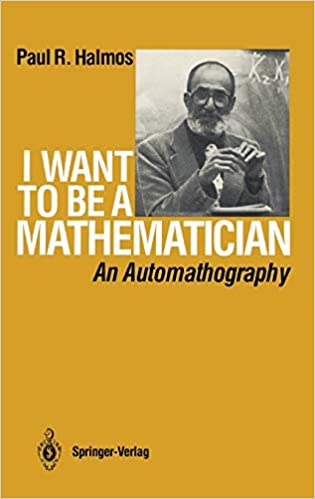
\includegraphics[width=\textwidth]{./img/Halmos_Mathematician}
\tcblower
\begin{boxQuote}{Paul Halmos}
    When a student comes and asks, "Should I become a mathematician?" the answer should be no.
    If you have to ask, you shouldn't even ask.
\end{boxQuote}
    \begin{boxQuote}{Paul Halmos}
    Don't just read it; fight it!
    Ask your own question, look for your own examples, discover your own proofs.
    Is the hypothesis necessary?
    Is the converse true?
    ... Where does the proof use the hypothesis?
    \end{boxQuote}
\end{boxResource}
%
\section{Textbooks}
\begin{boxResource}[lefthand width=5cm, sidebyside]{Hammack Book of Proof}
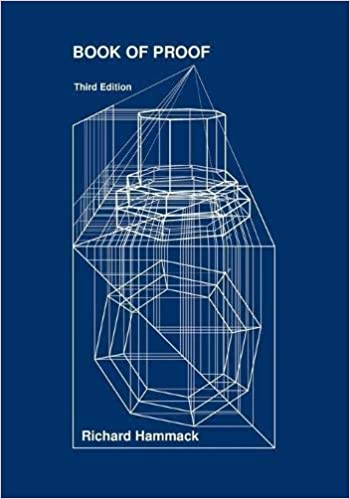
\includegraphics[width=\textwidth]{./img/Hammack_Proof}
\tcblower
Hammack's Book of Proof is a free online textbook that can be found \url{https://www.people.vcu.edu/~rhammack/BookOfProof/}.
It is also the highest quality introduction to rigorous mathematics that I have found, and \href{https://www.people.vcu.edu/~rhammack/BookOfProof/Adopters.html}{scores of colleges} seem to agree.
\end{boxResource}
%
\begin{boxResource}[lefthand width=5cm, sidebyside]{}
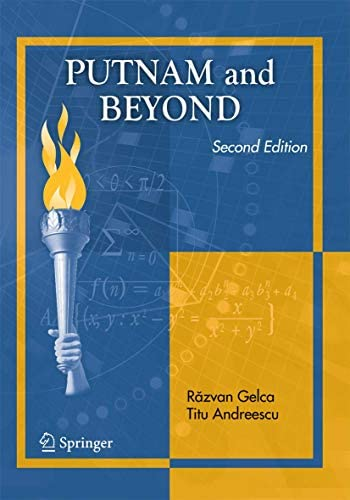
\includegraphics[width=\textwidth]{./img/Gelca_Putnam}
\tcblower
\begin{boxQuote}{Paul Halmos}
The heart of mathematics is its problems.
\end{boxQuote}
\end{boxResource}
%
\begin{boxResource}[sidebyside]{The Infinitely Large Napkin}
\begin{boxQuote}{Evan Chen}
The origin of the name “Napkin” comes from the following quote of mine.
    \begin{center}
        I’ll be eating a quick lunch with some friends of mine who are still in high school.  They’ll ask me what I’ve been up to the last few weeks, and I’ll tell them that I’ve been learning category theory. They’ll ask me what category theory is about. I tell them it’s about abstracting things by looking at just the structure-preserving morphisms between them, rather than the objects themselves. I’ll try to give them the standard example Grp, but then I’ll realize that they don’t know what a homomorphism is.  So then I’ll start trying to explain what a homomorphism is, but then I’ll remember that they haven’t learned what a group is. So then I’ll start trying to explain what a group is, but by the time I finish writing the group axioms on my napkin, they’ve already forgotten why I was talking about groups in the first place. And then it’s 1PM, people need to go places, and I can’t help but think: “Man, if I had forty hours instead of forty minutes, I bet I could actually have explained this all”.
    \end{center}
This book was initially my attempt at those forty hours, but has grown considerably since then.
\end{boxQuote}
\tcblower
Evan Chen is a Graduate Student at MIT who has been working on the Napkin for several years now.
The napkin touches every facet of undergraduate (and many parts of graduate) mathematics.
The latest version can be downloaded for free here: \url{https://web.evanchen.cc/napkin.html}
\end{boxResource}
%
\begin{boxResource}[lefthand width=5cm, sidebyside]{Gallian Algebra}
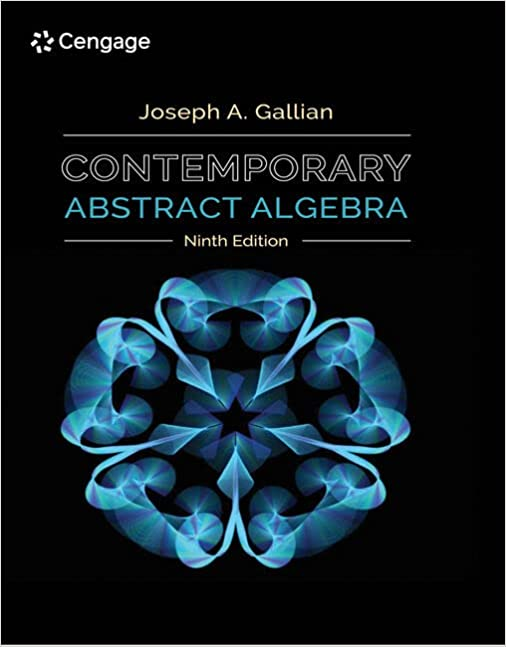
\includegraphics[width=\textwidth]{./img/Gallian_Algebra}
\tcblower
My favorite Algebra Book.
\end{boxResource}
%
\begin{boxResource}[lefthand width=5cm, sidebyside]{Judson Algebra}
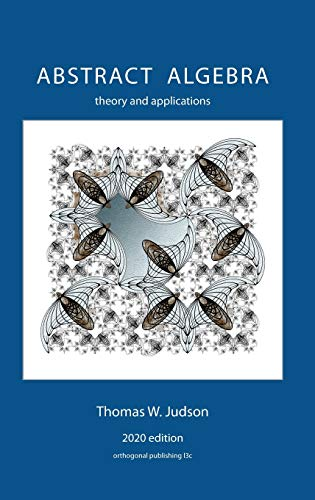
\includegraphics[width=\textwidth]{./img/Judson_Algebra}
\tcblower
This free (and open source) book can be found at \url{http://abstract.ups.edu/}.
\end{boxResource}
%
\begin{boxResource}[lefthand width=5cm, sidebyside]{}
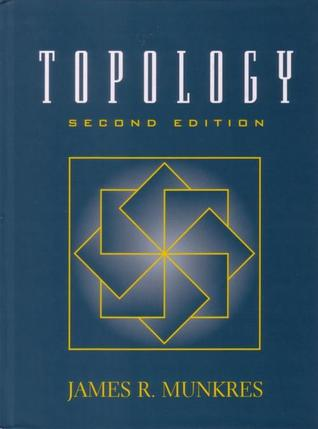
\includegraphics[width=\textwidth]{./img/Munkres_Topology}
\tcblower

\end{boxResource}
%
\section{Online Resources}
\begin{boxQuote}{Terry Tao}
I don't have any magical ability. I look at a problem, play with it, work out a strategy.
\end{boxQuote}
\begin{boxResource}[]{Terance Tao's Blog}
\url{https://terrytao.wordpress.com/}
\tcblower
Terry Tao is a fields medalist, and likely the best mathematician actively researching.
Thankfully for us mere mortals, he posts his thoughts and insights on a well-maintained blog.
\end{boxResource}
%
\begin{boxResource}{Borcherd's Lectures}
\url{https://www.youtube.com/channel/UCIyDqfi_cbkp-RU20aBF-MQ}
\tcblower
\href{https://www.ias.edu/ideas/2013/roberts-monster}{Richard Borcherds} is a Fields Medalist who, starting during the Pandemic, publishes his lectures online.
\end{boxResource}
%
\begin{boxResource}{MIT Open Course Ware}
\url{https://ocw.mit.edu/}
\end{boxResource}
%
\begin{boxResource}[lefthand width=5cm, sidebyside]{Strang Linear Algebra}
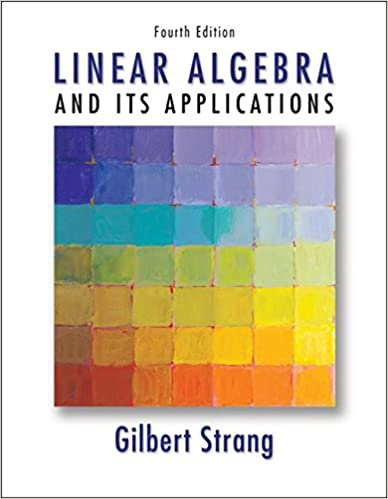
\includegraphics[width=\textwidth]{./img/Strang_Linear}
\tcblower
This is the best Linear Algebra Book.
Along with Strang's accompanying OCW Lectures,
    it is an indispensable resource for beginning engineers and mathematicians alike.
\end{boxResource}
%
\begin{boxResource}{Missing Semester}
\url{https://www.youtube.com/c/MissingSemester}
\tcblower
The thesis of the video series is that Computer Scientists are expected to use,
    but are never taught,
    a variety of tools,
    including:
\begin{itemize}
    \item \href{https://www.youtube.com/watch?v=a6Q8Na575qc}{Vim}
    \item \href{https://www.youtube.com/watch?v=Z56Jmr9Z34Q}{Bash}
    \item \href{https://www.youtube.com/watch?v=2sjqTHE0zok}{Git}
\end{itemize}
Mathematicians with a command over computers are sought after, both in Academia and Industry.
The series was taught by three Graduate Students at MIT.
\end{boxResource}
%
\begin{boxResource}{Sage Math}
\url{https://www.sagemath.org/}
\tcblower
An open source, mathematical superset of Python.
\end{boxResource}
%
\section{Problem Banks}
\begin{boxResource}{Yutsumura}
\url{https://yutsumura.com/category/group-theory/}
\end{boxResource}
%
\begin{boxResource}{Project Euler}
\url{https://projecteuler.net/}
\end{boxResource}
